\section{Codificador de Prioridade}

A tabela verdade para o Codificar de Prioridade 4x2 é apresentada em \ref{table:GrayTable}.

\begin{table}[!htb]
    \centering
    \caption{Tabela Verdade do Codificador de Prioridade 4x2}
    \begin{tabular}{cccc|cc}
        \toprule
        \textbf{$D_3$} & \textbf{$D_2$} & \textbf{$D_1$} & \textbf{$D_0$} & \textbf{$Y_1$} & \textbf{$Y_0$} \\
        \midrule
        0              & 0              & 0              & 0              & 0              & 0              \\
        0              & 0              & 0              & 1              & 0              & 0              \\
        0              & 0              & 1              & X              & 0              & 1              \\
        0              & 1              & X              & X              & 1              & 0              \\
        1              & X              & X              & X              & 1              & 1              \\
        \bottomrule
    \end{tabular}
    \label{tab:CodPriority}
\end{table}

Assim, o mapa de Karnaugh para  $Y_1$ é mostrado a seguir:

\begin{figure}[!ht]
\centering
\begin{karnaugh-map}[4][4][1][$D_0$][$D_1$][$D_2$][$D_3$]
\maxterms{0, 1, 3, 2}
\implicant{0}{2}
\end{karnaugh-map}
\caption{Mapa de Karnaugh para a saída $Y_1$ do Codificador de Prioridade 4x2.}
\end{figure}

Logo, pode-se expressar a saída $Y_1$ como:

\begin{equation}
    Y_1 = D_2 + D_3
\end{equation}

Já para $Y_0$, o mapa de Karnaugh é mostrado a seguir:

\begin{figure}[!ht]
\centering
\begin{karnaugh-map}[4][4][1][$D_0$][$D_1$][$D_2$][$D_3$]
\maxterms{0, 1, 4, 5, 7, 6}
\implicant{0}{5}
\implicant{4}{6}
\end{karnaugh-map}
\caption{Mapa de Karnaugh para a saída $Y_0$ do Codificador de Prioridade 4x2.}
\end{figure}

Logo, pode-se expressar a saída $Y_0$ como:

\begin{equation}
    Y_0 = (D_1 + D_3)(D_3 + \overline{D_2})
\end{equation}

Para o $A$, temos:

\begin{equation}
    A = D_3 + D_2 + D_1 + D_0
\end{equation}

Após isso, foi realizado o esquematico utilizando o software Quartus, resultando no esquemático mostrado na Figura \ref{fig:CodPriority}.

\begin{figure}[!ht]
    \centering
    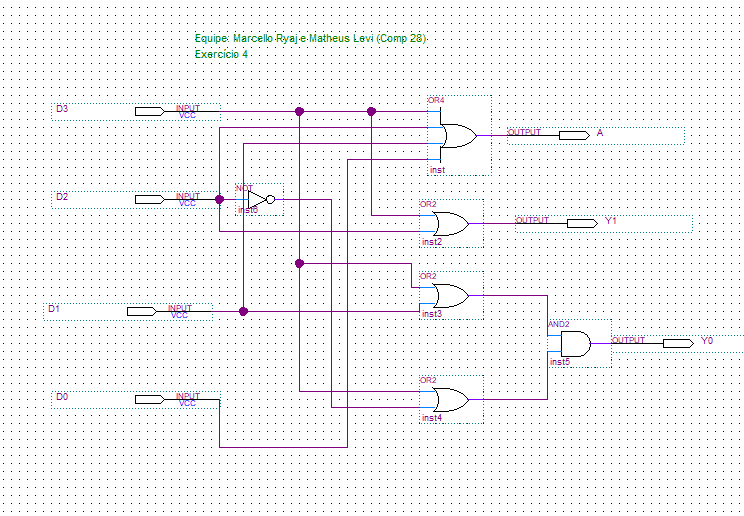
\includegraphics[width=0.8\textwidth]{fig/EsquematicoExercicio4.png}
    \caption{Diagrama esquemático do Codificador de Prioridade 4x2.}
    \label{fig:CodPriority}
\end{figure}

\newpage

Realizado o esquemático, foi feita a simulação funcional, resultando no diagrama de temporização mostrado na Figura \ref{fig:TempoCodPriority}.

\begin{figure}[!ht]
    \centering
    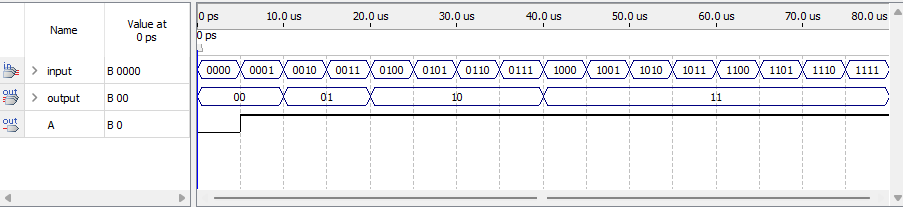
\includegraphics[width=1\textwidth]{fig/SimuExercicio4.png}
    \caption{Simulação funcional do Codificador de Prioridade 4x2.}
    \label{fig:TempoCodPriority}
\end{figure}

Ao comparar os resultados obtidos com a tabela verdade, percebe-se que o circuito implementado está de acordo com o esperado, apresentando as saídas corretas para cada combinação de entradas.


